%%%%%%%%%%%%%%%%%%%%%%%%%%%%%%%%
%% Ersetzen Sie in den folgenden Zeilen die entsprechenden -Texte-
%% mit den richtigen Werten.
\documentclass[course=erap]{aspdoc}
\usepackage{listings}
\usepackage{cite}
\usepackage{amssymb}
\usepackage{mathtools}
\usepackage{tkz-euclide}
\usepackage{subcaption}
\usepackage{algorithm}
\usepackage{algpseudocode}
\newcommand{\theGroup}{125} % Beispiel: 42
\newcommand{\theNumber}{A209} % Beispiel: A123
\author{Valentin Kostadinov, Mark Bley}
\date{\today}
%%%%%%%%%%%

% Diese Zeile bitte -nicht- aendern.
\title{Gruppe \theGroup{} -- Abgabe zu Aufgabe \theNumber}

\begin{document}
\maketitle

\section{Einleitung}
Die Hilbert-Kurve gehört zum Bereich der unendlichen Mathematik und bezeichnet
ein so genanntes Fraktal, also eine Kurve, die in der Theorie bis ins
Unendliche führt. Ihre Aufgabe ist es, möglichst effektive so viel Raum/Fläche
wie möglich zu \textit{besuchen}, d.h. es handelt sich um eine raumfüllende Kurve.
\newline

\begin{figure}[h]
    \centering
    \includegraphics[width=0.6\textwidth]{../img/hilbert-sample.png}
    \caption{2D Hilbert-Kurve}
\end{figure}

Sinn der Kurve ist dabei, sämtliche Koordinaten einer Fläche bzw eines Raumes
mit einer eindimensionalen Kurve abzudecken. Aufgrund des Aufbaus der Kurve
liegen hierbei Werte, die nahe beieinander auf der Kurve liegen, auch in
unmittelbarer Nähe auf der Fläche oder im Raum.  Diese Funktionalität macht die
Hilbert-Kurve für diverse Bereiche der Computer Wissenschaften sehr interessant
und kann zum Beispiel im Bereich der Parallelisierung der Simulation
physikalischer Prozesse verwendet
werden\cite{oberhofer}.
\newline
Die Aufgabe dieser Gruppe war es, im Verlauf des Praktikums die Erzeugung der
2-dimensionalen Hilbert-Kurve in Assembler zu implementieren.

\section{Problemstellung und Spezifikation}

Schon sehr bald nach Projektbeginn begann die Auseinandersetzung mit Ausgabe-
und Darstellungsmöglichkeiten für die generierte Hilbert-Kurve.
Nach einigem Überlegen wurde der Entschluss gefasst, sich auf die Hinweise der
Aufgabenstellung zu verlassen und die Kurvenkoordinaten in ein mittels C
generiertes SVG-Dokuments einzulesen und dieses auszugeben. Hierzu wurde
entschieden, das Dokument zeilenweise per fopen() einzulesen um Übersicht und
Anpassung zu erleichtern.
\newline
\newline
Die Wahl von SVG als Ausgabeformat bot sich zudem deshalb an, da einige
Mitglieder der Gruppe bereits grundlegende Kenntnisse im Umgang damit hatten,
was die Einarbeitung enorm erleichterte.
\newline
\newline
Um das fertige Dokument ohne weitere spezielle Programme einsehen zu können,
wurde weiterhin beschlossen, das SVG in eine HTML-Datei einzubetten, da diese
sich direkt im Browser öffnen ließen. 
Dies hatte den erfreulichen Vorteil, dass es das Testen der Ausgabe sehr
einfach und leicht überprüfbar machte. Dieser Aspekt machte sich gerade bei
Festlegen und Korrektur der Viewbox deutlich bemerkbar.
\newline
\newline
Problematisch war bei der Verwendung einzig die Tatsache, dass das
SVG-Koordinatensystem horizontal gespiegelt ist, d.h. (0,0) befindet sich in
der linken oberen Ecke und nicht in der linken unteren Ecke einer gegebenen
Fläche. Auch dieses Problem ließ sich mithilfe der Transformationsparameter (im
Spezifischen den Skalier- und Translationsparametern) ohne besonderen Aufwand
beseitigen.

\section{Lösungsfindung}
Als Eingabe haben wir die Zahl  $n\in\mathbb{N}$.

Die Hilbertkurve für den Basisfall $n=1$ entspricht einem Einheitsquadrat mit
der Länge ${\mathcal{L}}=2$ und den vier($2^{\mathcal{L}}=2^2=4$)
Basiskoordinaten $(0,0), (0,1), (1,1), (1,0)$.
Sei jetzt $n\in\mathbb{N}_{>1}$, so entspricht die Hilbertkurve des Grades $n$
einem Einheitsquadrat der Länge ${\mathcal{L}}=2(n-1)$ mit
$2^{\mathcal{L}}=2^{2(n-1)}=4^{n-1}$ Koordinaten.
Im Weiteren arbeiten wir mit unserer Eingabe $k_{n}=2^n$ und betrachten
$k_{n>1}$, da $n=1$ dem Basisfall entspricht.
Es ist hilfreich, es klar zumachen, dass sich jedes Einheitsquadrat $k_{n}$ in
$4k_{n-1}$ Einheitsquadrate aufteilen lässt(beim Aufbau von $k_{n}$)

\begin{figure}[h]
    \centering
    \includegraphics[width=0.35\textwidth, height=0.12\textheight]{../img/hblocks.png}
    \caption{Aufteilung der Einheitsquadrate}
\end{figure}

Es ist ersichtlich, dass Bereiche $B$ und $C$ des Einheitsquadrates $k_{n}$
lediglich eine Verschiebung von dem $k_{n-1}$ Einheitsquadrat darstellen und
die Richtung erhalten bleibt. Somit gilt dass die Koordinaten des Bereiches $B$
sind:\\
$x\_coord(k_{n})=x\_coord(k_{n-1})$\\
$y\_coord(k_{n})=y\_coord(k_{n-1})+k_{n-1}$

Analog dazu, gilt für den Bereich $C$:\\
$x\_coord(k_{n})=x\_coord(k_{n-1})+k_{n-1}$\\
$y\_coord(k_{n})=y\_coord(k_{n-1})+k_{n-1}$

Der Bereich $A$ wird von einer Verschiebung(um $x:=0$ und $y:=0$) und einer
Achsensymmetrie entlang der Diagonale gebildet.

\begin{figure}[H]
    \centering
    \includegraphics[width=0.35\textwidth,  height=0.12\textheight]{../img/BereichA.png}
    \caption{Achsensymmetrie entlang der Diagonale - Bereich $A$}
\end{figure}

Bei dieser Symmetrie(im Rahmen des Einheitsquadrates)werden die $x$ und $y$
Koordinaten lediglich getauscht($siehe$ Abbildung  5). Somit gilt für den
Bereich $A$:\\
$x\_coord(k_{n})=y\_coord(k_{n-1})$\\
$y\_coord(k_{n})=x\_coord(k_{n-1})$

Der Bereich $D$ wird auch von einer Verschiebung(um $x:=k_{n-1}$ und $y:=0$)
und einer Achsensymmetrie entlang der zweiten Diagonale gebildet.

\begin{figure}[H]
    \centering
    \includegraphics[width=0.35\textwidth, height=0.12\textheight]{../img/BereichD.png}
    \caption{Achsensymmetrie entlang der anderen Diagonale - Bereich $D$}
\end{figure}

Dabei  werden $x=(k_{n-1}-1)-y$ und $y=(k_{n-1}-1)-x$ ($siehe$ Abbildung  5).
Zusätzlich dazu müssen wir den Bereich $B$ um $k_{n-1}$ nach rechts schieben.
Somit gilt für den Bereich $D$:\\
$x\_coord(k_{n})=(k_{n-1}-1)-y\_coord(k_{n-1})+k_{n-1}$\\
$y\_coord(k_{n})=(k_{n-1}-1)-x\_coord(k_{n-1})$

\begin{figure}[H]
\centering
\begin{subfigure}{.5\textwidth}
  \centering
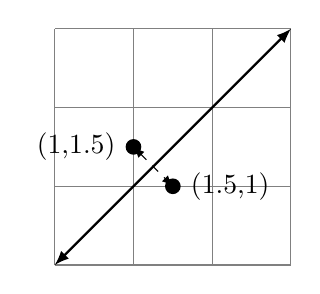
\begin{tikzpicture}
   \tkzInit[xmax=3,ymax=3,xmin=0,ymin=0]
   \tkzGrid
   \tkzAxeXY
   \draw[ thick,latex-latex] (0,0) -- (3,3);
   \node[label={180:{(1,1.5)}}, circle,fill,inner sep=2pt] at (1, 1.5){};
   \draw[dashed,latex-latex] (1,1.5) -- (1.5,1);
   \node[label={0:{(1.5,1)}}, circle,fill,inner sep=2pt] at (1.5, 1){};
  \end{tikzpicture}
  \caption{Erste Diagonale}
\end{subfigure}%
\begin{subfigure}{.5\textwidth}
  \centering
    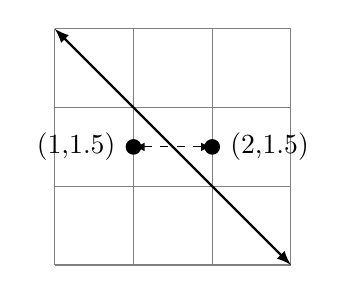
\begin{tikzpicture}
   \tkzInit[xmax=3,ymax=3,xmin=0,ymin=0]
   \tkzGrid
   \tkzAxeXY
   \draw[ thick,latex-latex] (0,3) -- (3,0);
   \node[label={180:{(1,1.5)}}, circle,fill,inner sep=2pt] at (1, 1.5){};
   \draw[dashed,latex-latex] (1,1.5) -- (2,1.5);
   \node[label={0:{(2,1.5)}}, circle,fill,inner sep=2pt] at (2, 1.5){};
  \end{tikzpicture}
  \caption{Zweite Diagonale}
\end{subfigure}
\caption{Symmetrie entlang der Diagonalen}
\end{figure}


Jetzt kommen wir zur Repräsentation der $k_{n}*k_{n}=2^n*2^n=2^{2n}=4^n$ Zahlen
im Einheitsquadrat. Die Koordinaten des Basisfalls lauten: $(0,0), (0,1),
(1,1), (1,0)$.\\ Unser Ziel ist es jetzt den Fall $k_{2}$ zu behandeln, ihn
mithilfe unserer bisherigen Überlegungen auf den Basisfall zurückzuführen und
dann zu schließen, dass es für alle $k_{n}$ gilt.\\

\begin{figure}[H]
\centering
\begin{subfigure}{.5\textwidth}
\centering
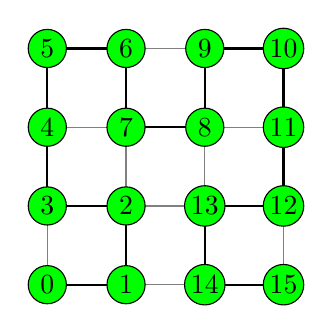
\begin{tikzpicture}
   \tkzInit[xmax=3,ymax=3,xmin=0,ymin=0]
   \tkzGrid
   \tkzAxeXY
   \draw[ thick,latex-latex] (0,0) -- (1,0);
   \draw[ thick,latex-latex] (1,0) -- (1,1);
   \draw[ thick,latex-latex] (1,1) -- (0,1);  
   \draw[ thick,latex-latex] (0,1) -- (0,2);
 \draw[ thick,latex-latex] (0,2) -- (0,3);
 \draw[ thick,latex-latex] (0,3) -- (1,3);
 \draw[ thick,latex-latex] (1,3) -- (1,2);
 \draw[ thick,latex-latex] (1,2) -- (2,2);
 \draw[ thick,latex-latex] (2,2) -- (2,3);
  \draw[ thick,latex-latex] (2,3) -- (3,3);
 \draw[ thick,latex-latex] (3,3) -- (3,2);
 \draw[ thick,latex-latex] (3,2) -- (3,1);
 \draw[ thick,latex-latex] (3,1) -- (2,1);
 \draw[ thick,latex-latex] (2,1) -- (2,0);
 \draw[ thick,latex-latex] (2,0) -- (3,0);
 
   \node[fill=green,circle,inner sep=2pt, draw] at (0, 0){0};
   \node[fill=green,circle,inner sep=2pt, draw] at (1, 0){1};
   \node[fill=green,circle,inner sep=2pt, draw] at (1, 1){2};
   \node[fill=green,circle,inner sep=2pt, draw] at (0, 1){3};
   
   \node[fill=green,circle,inner sep=2pt, draw] at (0, 2){4};
   \node[fill=green,circle,inner sep=2pt, draw] at (0, 3){5};
   \node[fill=green,circle,inner sep=2pt, draw] at (1, 3){6};
   \node[fill=green,circle,inner sep=2pt, draw] at (1, 2){7};
   
   \node[fill=green,circle,inner sep=2pt, draw] at (2, 2){8};
   \node[fill=green,circle,inner sep=2pt, draw] at (2, 3){9};
   \node[fill=green,circle,inner sep=1pt, draw] at (3, 3){10};
   \node[fill=green,circle,inner sep=1pt, draw] at (3, 2){11};
   
   \node[fill=green,circle,inner sep=1pt, draw] at (3, 1){12};
   \node[fill=green,circle,inner sep=1pt, draw] at (2, 1){13};
   \node[fill=green,circle,inner sep=1pt, draw] at (2, 0){14};
   \node[fill=green,circle,inner sep=1pt, draw] at (3, 0){15};
\end{tikzpicture}
\end{subfigure}%
\begin{subfigure}{.5\textwidth}
\centering
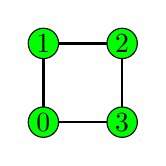
\begin{tikzpicture}
   \tkzInit[xmax=1,ymax=1,xmin=0,ymin=0]
   \tkzGrid
   \tkzAxeXY
   \draw[ thick, latex-latex] (0,0) -- (0,1);
   \draw[ thick,latex-latex] (0,1) -- (1,1);
   \draw[ thick,latex-latex] (1,1) -- (1,0);
   \draw[ thick,latex-latex] (1,0) -- (0,0);
   \node[fill=green,circle,inner sep=1pt, draw] at (0, 0){0};
   \node[fill=green,circle,inner sep=1pt, draw] at (0, 1){1};
   \node[fill=green,circle,inner sep=1pt, draw] at (1, 1){2};
   \node[fill=green,circle,inner sep=1pt, draw] at (1, 0){3};
\end{tikzpicture}
\end{subfigure}%
\begin{subfigure}{.5\textwidth}
  \centering
\begin{table}[H]
\begin{tabular}{|c| c| c|}
\hline
01 &  10 \\ 
\hline
00 & 11\\
\hline
\end{tabular}
\end{table}
\end{subfigure}%
  \caption{Reihenfolge der Basiskoordinaten und die Bitrepräsentation}
\end{figure}

Das Einheitsquadrat $k_{2}$ besteht aus $k_{2}*k_{2}=2^2*2^2=16$ Koordinaten.
Jede Zahl vom $k_{2}$ lässt sich durch $\log_2 16=4$ Bits repräsentieren.
Weiter unterteilen wir das Einheitsquadrat in die schon definierte Bereiche $A,
B, C$ und $D$ wie folgt: $\{0,1,2,3\}\in A; \{4,5,6,7\}\in B; \{8,9,10,11\}\in
C; \{12,13,14,15\}\in D$. Darüber hinaus bemerken wir, dass die Zahlen folgende
Bitrepräsentationen besitzen:

Für $A$ gilt: 
\begin{tabular}{|c| c|}
\hline
00 &  xx \\ 
\hline
\end{tabular}\\
Für $B$ gilt: 
\begin{tabular}{|c| c|}
\hline
01 &  xx \\ 
\hline
\end{tabular}\\
Für $C$ gilt: 
\begin{tabular}{|c| c|}
\hline
10 &  xx \\ 
\hline
\end{tabular}\\
Für $D$ gilt: 
\begin{tabular}{|c| c|}
\hline
11 &  xx \\ 
\hline
\end{tabular}

Diese Konfiguration beschreibt aber genau den Pfad beim Basisfall. Weiter
erinnern wir uns daran, dass sich Bereiche $B$ und $C$ aus einer Verschiebung
vom $k_{1}$ herleiten lassen. Das bedeutet, dass die unteren 2 Bits der Zahlen
im Bereich $B$ vom $k_{2}$ (mit xx markiert) den Bitrepräsentationen der
jeweilig verschobenen Zahlen im Basisfall gleichen. Z.b sind $7=0111b$ und
$3=0011b$. In dem Falle werden die um $x:=0$ und $y:={k_{1}}$ verschoben.\\
Analog gilt eine Verschiebung um $x:={k_{1}}$ und $y:={k_{1}}$ für den Bereich
$C$, wobei auch hier die unteren 2 Bits gleich bleiben. Z.b sind $10=1010b$ und
$2=0010b$.\\ Für die Bereiche $A$ und $D$ müssen wir auch die Symmetrie entlang
der Diagonale und die Verschiebung (im Falle von $D$) auch miteinbeziehen. So
entspricht z.B $1=0001b\in A$ wegen den letzten beiden Bits der $1$ vom
$k_{1}$, welche oben links steht. Nach der Symmetrie entlang der Diagonale aber
geht diese $1$  vom $k_{1}$ rechts unten mit Koordinaten $(1,0)$. Analoges gilt
für den Bereich $D$, wo aber die Symmetrie entlang der zweiten Diagonale
passiert und es eine Verschiebung auf der x-Achse um $k_{1}$ besteht.\\ Für
$n>2$ konnten wir solange zurückführen, bis wir den Basisfall erreichen. Die
Bereiche werden natürlich laut Definition aus der vorherigem Einheitsquadrat
gebildet.\\ Kommen wir jetzt zur iterativen Implementierung des Algorithmus.\\
Wie schon erwähnt, besteht eine Hilbertkurve des Grades n aus
$k_{n}*k_{n}$=$2^n*2^n=2^{2n}=4^n$ Zahlen, deren Koordinaten zu bestimmen sind.

\begin{algorithm}[H]
\caption{Koordinate für jede Zahl}
\begin{algorithmic}[1]
\ForAll{$i:=0 < 4^n$}
    \State \Call {hindex2xy}{i, $2^n$}
\EndFor
\end{algorithmic}
\end{algorithm}
\begin{algorithm}[H]
\caption{Finde letzte beide Bits}
\begin{algorithmic}[1]
\Function {last2bits}{$x$}
	\State \Return $x$ \& $3$
\EndFunction
\end{algorithmic}
\end{algorithm}
\begin{algorithm}[H]
\caption{Berechne die Koordinaten für die Zahl $hindex$}
\begin{algorithmic}[1]
\Function {hindex2xy}{$hindex$,$N$}
	\State $positions:=[ [0, 0],[0, 1],[1, 1],[1, 0] ]$
	\State $x:=positions[\Call{last2bits}{$hindex$}][0]$
	\State $y:=positions[\Call{last2bits}{$hindex$}][1]$
	\State $hindex:= hindex >> 2$
	\ForAll{$n:=4; <= N; n:=n<<2$}
    		\State $n2:=n/2$
		\If {\Call{last2bits}{$hindex$}=0}
			\State $tmp:=x; x:=y; y:=tmp$
		\ElsIf {\Call{last2bits}{$hindex$}=1}
			\State $y:=y+n2$		
		\ElsIf {\Call{last2bits}{$hindex$}=2}
			\State $x:=x+n2; y:=y+n2$	
		\ElsIf {\Call{last2bits}{$hindex$}=3}
			\State $tmp:=y; y:=(n2-1)-x; x:=(n2-1)-tmp+n2$	
		\EndIf			
		\State $hindex:=hindex>>2$
	\EndFor
	\State \Return [x, y]
\EndFunction
\end{algorithmic}
\end{algorithm}

\section{Dokumentation der Implementierung}

Das Projekt haben wir, wie folgt in 4 Segmente aufgeteilt:
\begin{itemize}
    \item \ref{arg_parse}   \lstinline{arg_parse}
    \item \ref{file_helper} \lstinline{file_helper}
    \item \ref{hilbert}     \lstinline{hilbert}
    \item \ref{main}        \lstinline{main}
\end{itemize}

\subsubsection{\lstinline{arg_parse}}\label{arg_parse}
Dies ist nur eine einfache Klasse bei der wir die Funktionen die sich um das
Parsen der Argumente kümmern eingebettet haben. Sie besteht aus einer Funktion
\lstinline{print_help}, die wie der Name schon sagt, einfach nur eine Nachricht
ausgibt die, die Benutzung des Programms erläutert.

\begin{lstlisting}[numbers=none,caption={Output von print\_help},label={usage},belowcaptionskip=0.6cm]
./main [-h] [-t] [-d n] [-f <name>] [-c] -- prints the Nth grade of the hilbert curve to an svg/html file

where:
	-h  show this help text
	-f  outputs the svg to specified file name
	-d  degree of the hilbert curve (default 2)
	-c  if set uses c implementation (default uses assembler)
	-t  if set creates an html file of the sv
\end{lstlisting}

In \lstinline{arg_parse.h} auch enthaltene Funktion ist die Funktion:
\begin{lstlisting}[caption={Signatur von arg\_parse},belowcaptionskip=0.6cm]
void arg_parse(int argc,                // stores # of arguments
               char** argv,             // store value of arguments
               char** filename,         // name of output file
               int* n,                  // degree of hilbert curve
               short* c,                // c-flag, if set uses c algorithm
               short* html);            // html-flag, if set outputs an html doc
\end{lstlisting}

Wie der Name schon darauf hin deutet ist die Aufgabe dieser Funktion das Parsen
der über die Kommandozeile übergebene Argumente. Diese Funktion vergewissert
auch das gültige Werte als Grad für die Hilbert Kurve übergeben wurde. Wurde
kein gültiger Wert übergeben so wird der Default Wert 1 genommen.

\subsubsection{\lstinline{file_helper}}\label{file_helper}
Hier enthaltene Funktionen sind für das Outputen der Ergebnisse in die Ziel
Dateien, so wie für den Umgang mit Strings zuständig. \newline

Die Funktion \lstinline{to_svg} bekommt den Namen den die erzeugte Datei
erhalten soll.  Den Grad der Funktion sowie zwei Listen mit den jeweiligen x-,
bzw. y-Koordinaten der Funktion. Außerdem wird noch das \lstinline{html} Flag
übergeben, dass entscheidet ob eine HTML-Datei erzeugt werden soll oder direkt
eine SVG. Diese Funktion war \textbf{nicht} gefordert fanden wir aber zum
darstellen/anzeigen der Graphen sehr hilfreich, da man einfach mit seinem
Browser der Wahl sich die Kurve anschauen kann.

\begin{lstlisting}[caption={Signatur von to\_svg},belowcaptionskip=0.6cm]
void to_svg(char* filename,     // name of output file
        unsigned int degree,    // degree of hilbert curve
        unsigned int* x,        // x-coordinates of hilbert curve
        unsigned int* y,        // y-coordinates of hilbert curve
        short html);            // html flag, if set outputs an html file
\end{lstlisting}

Die Funktion \lstinline{str_append} kriegt zwei Strings, fügt diese zusammen
und gibt den resultieren String dann zurück. Diese Funktion ist nur eine
Hilfsfunktion um Code Wiederholungen zu vermeiden, ist nicht Teil der
geforderten Aufgabe.

\begin{lstlisting}[caption={Signatur von str\_append},belowcaptionskip=0.6cm]
char* str_append(char* s1, char* s2);
\end{lstlisting}

Letztlich noch gibt es die Funktion \lstinline{file_ending} die den Dateiname
kriegt und den HTML-Falg und je nach dem ob dieser gesetzt wurde wird am ende
des Dateinames \lstinline{.html} oder \lstinline{.svg} angehängt.

\begin{lstlisting}[caption={Signatur von file\_ending},belowcaptionskip=0.6cm]
char* file_ending(char*filename, short html);
\end{lstlisting}

\subsubsection{\lstinline{hilbert}}\label{hilbert}
In diesen Dateien befindet sich der eigentliche Alogrithmus zum erzeugen der
Hilbert Kurven.  Zum einen gibt es die C-Variante, diese ist, zur Einfachheit,
in 2 Methoden aufgeteilt.  Die erste Aufgerufene Methode \lstinline{hilbert_c}
ist die Methode so wie diese von der Aufgabe gefordert wurde. Diese erhält den
Grad der Kurve, sowie zwei Pointer auf die x-Koordinaten und y-Koordinaten.

\begin{lstlisting}[caption={Signatur von hilbert\_c},belowcaptionskip=0.6cm]
void hilbert_c(unsigned int degree,     // degree of hilbert curve
               unsigned int* x,         // x-coordinates of hilbert-curve
               unsigned int* y);        // y-coordinates of hilbert-curve
\end{lstlisting}

In der Klasse ist außerdem noch ein \lstinline{struct point} definiert
das helfen soll die Koordinaten zwischen zu speichern. Dieses struct besteht nur
aus 2 Integern, x und y. \newline
Die Funktion \lstinline{hindex2xy} bekommt den Index von einem Punkt in der
Hilbert Kurve sowie den Grad der Kurve und gibt ein Punkt zurück mit den
2-Dimensionalen Koordinaten des Indices.
\begin{lstlisting}[caption={Signatur von hindex2xy},belowcaptionskip=0.6cm]
point_t* hindex2xy(int hindex, int n);
\end{lstlisting}
Letztendlich in der \lstinline{hilbert.S} Datei ist der egentliche
x86-Assembler Hilbert Algorithmus implementiert der von der Aufgabe gefordert
war. Die Signatur befindet sich in der \lstinline{main.c} und lautet wie folgt:

\begin{lstlisting}[caption={Signatur von hilbert},belowcaptionskip=0.6cm]
extern void hilbert(unsigned int degree,     // degree of hilbert curve
                    unsigned int* x,         // x-coordinates
                    unsigned int* y);        // y-coordinates
\end{lstlisting}

\subsubsection{\lstinline{main}}\label{main}
Wie der Name schon sagt liegt in dieser Datei auch die \lstinline{main}
Funktion die alles aus den anderen Klassen zusammen bringt.

\subsection{Usage}
Der Code um die Hilbert Kurven zu generieren liegt im Verzeichnis
\lstinline{./src/} . Das Programm lässt sich mittels einem \lstinline{Makefile}
kompilieren. Die ausführbare Datei liegt dann im Unterverzeichnis
\lstinline{./bin/main}. Das einfache Ausführen (ohne Argumente) des Programms
erzeugt eine SVG-Datei mit einer Hilbert Kurve ersten Grades. Das Programm
kann man in Verbindung mit dem beiliegenden \lstinline{run.sh} benutzten was das
die Ausführung des Programms vereinfacht und die generierten SVG- sowie
HTML-Dateien in den \lstinline{./output/} Ordner legt.
Eine Beispiel Ausführung wäre:

\begin{lstlisting}[numbers=none,caption=Beispiel Ausführung,belowcaptionskip=0.6cm]
./run.sh -d 5 -f foo -t
\end{lstlisting}


Dieser Befehlt erzeugt eine Hilbert Kurve des fünften Grades und speichert
diese als HTML-Datei wie folgt: \lstinline{./output/foo_5.html} . Siehe
\ref{usage} für weitere Details.


\section{Ergebnisse}
Was wir natürlich bemerkt haben war der Unterschied von unserer C
Implementierung zu unserer x86-Assembler Implementierung. Bei kleinen Graden (1
- 9) für eine Hilbert Kurve erkennt man kaum den Unterschied zwischen den beiden
Varianten. Erhöht man jedoch den Grad der Kurve kommt es zu erheblichen
Unterschieden zur Laufzeit wie es sich im folgend Graph erkennen lässt.
\begin{figure}[H]
    \label{fig:results}
    \centering
    \includegraphics[width=0.6\textwidth]{../img/result-plot.png}
    \caption{Laufzeit von X86-Assembler gegen C Variante}
\end{figure}

Da wir unser Programm so ausgestattet haben das man entweder die C Variante oder
die x86-Assembler Variante zur Laufzeit benutzen kann, mussten wir alles nur
einmal kompilieren. Das Programm wurde mit dem GCC-Falg \lstinline{-O2}
kompiliert, um die \textit{best möglichste Laufzeit}\cite{gcc-optimazation} zu
erzielen und durch das gleiche getestet. Wie man aus dem obigen Graph
\ref{fig:results} gut erkennt ist bei höheren Graden (13) die Laufzeit von der
x86-Assembler Implementierung doppelt so niedrig wie bei der C-Variante.

\subsection{Testverfahren}
Zum Testen des Programms haben wir erstmal ein Output der Laufzeit gebraucht.
Diesen haben wir mit der Funktion \lstinline{clock} aus \lstinline{time.h}
gemessen.
\begin{lstlisting}[language=c,caption={Zeitmessung des Algorithmus},belowcaptionskip=0.6cm]
    start = clock();
    hilbert(n, x_points, y_points);
    end = clock();
    cpu_time_used = ((double) (end - start)) / CLOCKS_PER_SEC;
    printf("%.5f\n", cpu_time_used);
\end{lstlisting}

Wir haben einfach vor und nach dem Ablaufen des Algorithmus die Zeit gemessen,
dann jeweils Endzeit minus Startzeit um die eigentlich verbrauchte Zeit des
Algorithmus zu messen.

In einem Python Script haben wir dann beide Verfahren von einem Start Grad bis
zum einem End Grad laufen lassen. Um Fehler zu minimieren haben wir dann jeden
Grad mehrmals ausgeführt und dann einen Durchschnitt für jeden einzelnen Grad
erstellt.

\begin{lstlisting}[language=python,caption={Durchschnittszeit Berechnung},belowcaptionskip=0.6cm]
            avg = 0.0
            prog = ['./bin/main_test', '-d10']
            '''
            runing some more times to have an average
            and rule out errors
            '''
            for k in range(0, extra_loops):
                avg += float(subprocess.check_output(prog))
            avg = avg / extra_loops
            avg_time.append(avg)
\end{lstlisting}
Für weitere Details wie die ganze Testumgebung aufgebaut ist sollte man sich
das Script \lstinline{run-tests.py} im Verzeichnis \lstinline{tests} anschauen.
Dieses Script generiert auch eine Datei (\lstinline{c-vs-ass-output}) in dem die
Durchschnittszeiten der beiden Varianten stehen. Mit dieser Datei kann man mit
einem Plot-Programm seiner Wahl (in unserem Fall haben wir uns für Gnuplot
entschieden), z.B. den obigen Graph \ref{fig:results} darstellen. Die
Plot-Konfiguration um den Graph zu erstellen, so wie ein Script
\lstinline{run.sh}, was alle Schritte für einen erledigt sind auch im Ordner
enthalten


\section{Zusammenfassung}
Der von uns implementierte Algorithmus, für die Berechnung der Hilbert-Kurve,
ist der Iterative.  Neben diesem existiert noch eine Rekursive Möglichkeit den
Algorithmus zu implementieren, jedoch ist bei größeren Graden der Stack
ziemlich schnell voll im Gegensatz zur Iterativen Variante. \newline
Wir haben uns gegen die Verwengund der SIMD Befehle entschlossen, da wir
Iterativ immer nur mit einem, bzw zwei (2 Koordinate x und y), Werten
gleichzeitig Arbeiten.  Deshalb ist die Verwendung der SIMD Befehele eher
ungünstig da wir diese nie richtig ausnutzen.

\bibliography{mybib}{}
\bibliographystyle{plain}
\end{document}
